\section{Results}

The controllers have been simulated in MATLAB Simulink in order to generate results presented in this section. 

The model parameters can be seen in \autoref{ParametersQuadcopter}. All of them have been obtained through test except for the moments of inertia, which were calculated by following an analytical procedure.

\begin{table}[H]
    \centering
    \begin{tabular}{c|c|c}
        %------------------------------------------------------------------------------------------
        \textbf{Symbol} &\textbf{Value} &\textbf{Units}\\
        \hline %-----------------------------------------------------------------------------------
        $m$ & 0.996       &kg\\
        \hline %-----------------------------------------------------------------------------------
        $L$  &   0.225       & m\\
        \hline %-----------------------------------------------------------------------------------
        $J_x$  & 0.01073       & \si{kg \  m^2}\\
        \hline %-----------------------------------------------------------------------------------
        $J_y$  & 0.01073       & \si{kg \  m^2}\\
        \hline %-----------------------------------------------------------------------------------
        $J_z$  & 0.02135       & \si{kg \  m^2}\\
        \hline %-----------------------------------------------------------------------------------
        $k_{th}$  & $1.32922\cdot10^{-5}$       & \si{N \  s^2 \  rad^{-2}}\\
        \hline %-----------------------------------------------------------------------------------
        $k_{d}$  & $9.39741 \cdot10^{-7}$       & \si{N \  m \  s^2 \  rad^{-2}}\\
        \hline %-----------------------------------------------------------------------------------
        $\overline{\omega}_i$& 429      & \si{rad \ s^{-1}}\\
        
    \end{tabular}
    \caption{Parameters used though the analysis and design.}
    \label{ParametersQuadcopter}
\end{table}
The attitude controller is defined by the chosen feedback, integral poles, $[-6.0, -6.2, -6.4, -6.6, -6.8, -7.0, -7.2, -7.4, -7.6]$, and  the observer poles, $[-20, -25, -30]$.

The translation velocity controllers for x and y are $C_{\dot{x}}(s)= -0.1$, $C_{\dot{y}}(s)= 0.1$ and the position ones are $C_x(s)= 0.5$, $C_y(s)= 0.5$. The PI-controller for the z translational velocity is $C_{\dot{z}}(s)=-201\frac{s+0.8}{s}$ and the outer loop P-controller is $C_z=0.9$.

These controllers are discretized using the Tustin method with a sampling period of 35 ms due to the 

Regarding the network, the mean delay is 30 ms and the package loss probability is set to 0 due to the low sending frequency used in the system.
The simulation results obtained with these parameters and controllers are shown in \autoref{PositionControl}.
\begin{figure}[H]
	\centering
	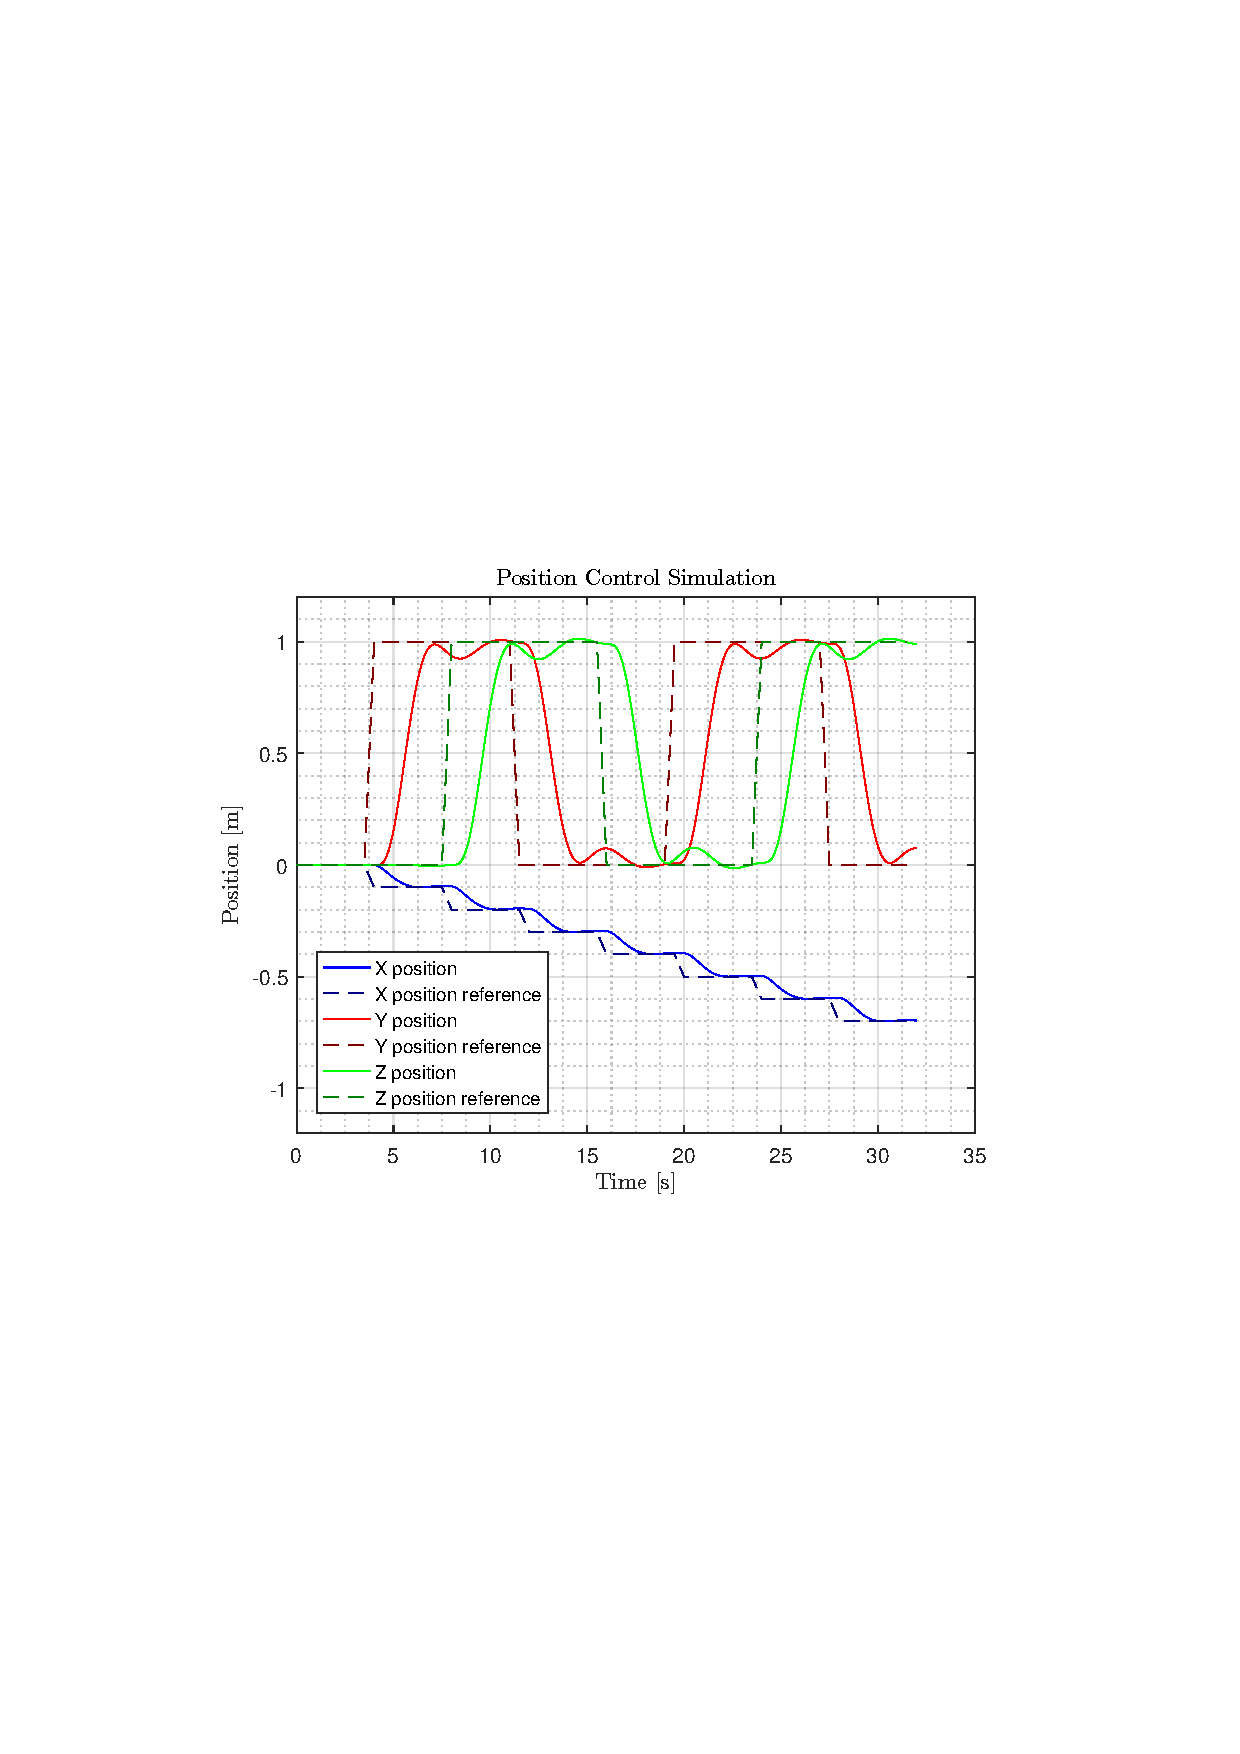
\includegraphics[scale=0.5]{figures/PositionControl}
	\caption{Position control results in the three inertial axes directions. The references given to the control system are shown with dashed lines.}
	\label{PositionControl}
\end{figure}

The inner attitude controller results are also included and shown in \autoref{AttitudeControl} so the performance of the attitude control can be evaluated. 
\begin{figure}[H]
	\centering
	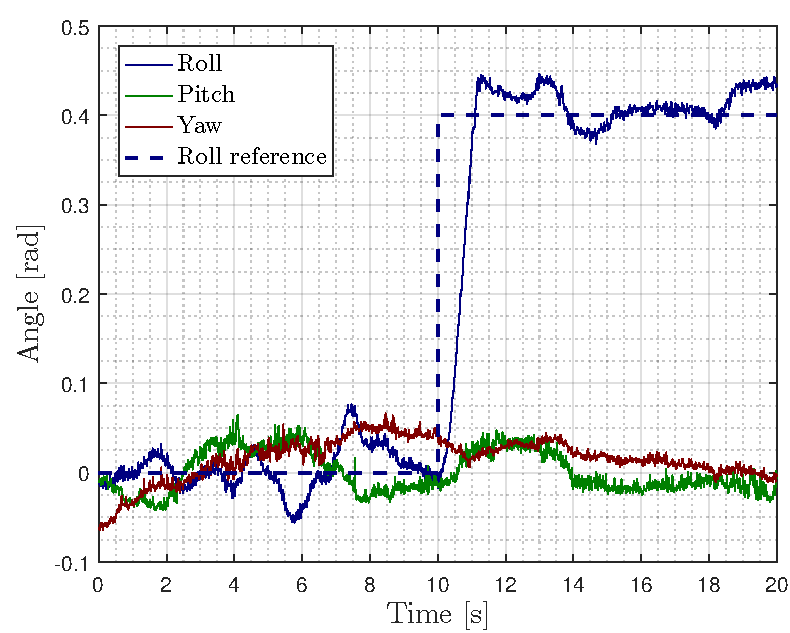
\includegraphics[scale=0.5]{figures/AttitudeControl}
	\caption{Attitude control results in the three angles. The references given to the attitude control system are shown with dashed lines.}
	\label{AttitudeControl}
\end{figure}


